\section{Perintah Navigasi}

\subsection{Installing Python And Anaconda}
\begin{enumerate}
  \item Download dan instal Python terbaru, versi 3.7.2
  \item Setelah selesai instal Python, download dan instal aplikasi Anaconda.
  \item Instal Anaconda dengan klik kanan aplikasi Anaconda.exe yang telah didownload tadi, kemudian Run as administrator. 
      \begin{figure}[!ht]
	  \centering
	  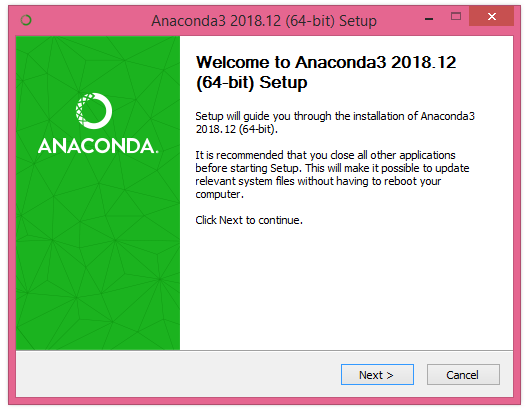
\includegraphics[scale=0.4]{figures/instal/1.PNG}
	  \caption{Instalasi Anaconda Proses 1}
	  \label{labelgambar2}
	  \end{figure}
  \item Kemudian pilih next (pada gambar \ref{labelgambar2}).
	 \begin{figure}[h]
	  \centering
	  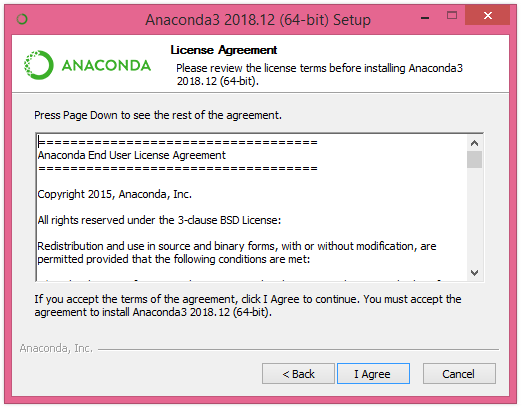
\includegraphics[scale=0.4]{figures/instal/2.PNG}
	  \caption{Instalasi Anaconda Proses 2}
	  \label{labelgambar3}
	  \end{figure}
  \item Kemudidan pilih I Agree (pada gambar \ref{labelgambar3}).
\begin{figure}[h!]
	  \centering
	  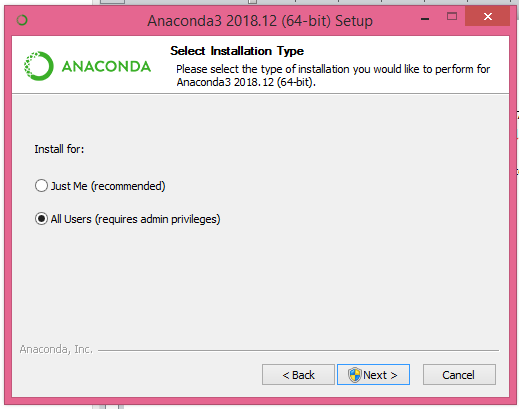
\includegraphics[scale=0.4]{figures/instal/3.PNG}
	  \caption{Instalasi Anaconda Proses 3}
	  \label{labelgambar4}
	  \end{figure}
  \item Pilih All User. kemudian klik Next (pada gambar \ref{labelgambar4}).
\begin{figure}[h!]
	  \centering
	  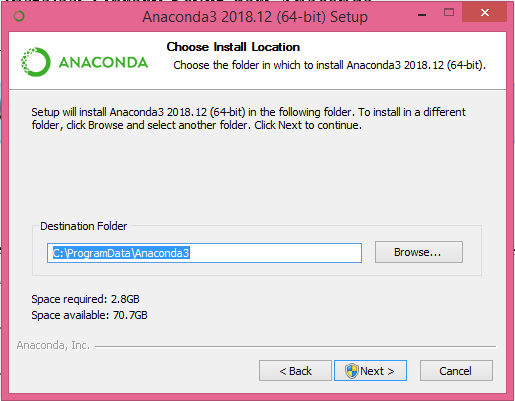
\includegraphics[scale=0.4]{figures/instal/4.PNG}
	  \caption{Instalasi Anaconda Proses 4}
	  \label{labelgambar5}
	  \end{figure}
  \item Tentukan directory instalasi. saya sarankan biarkan default saja. kemudian next (pada gambar \ref{labelgambar5}).
\begin{figure}[h!]
	  \centering
	  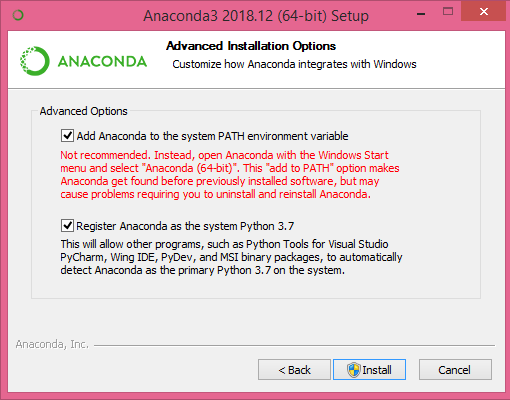
\includegraphics[scale=0.4]{figures/instal/5.PNG}
	  \caption{Instalasi Anaconda Proses 5}
	  \label{labelgambar6}
	  \end{figure}
  \item Kemudian centang pilihan Add Anaconda to the system PATH. kemudian pilih instal. Tunggu hingga proses instal selesai (pada gambar \ref{labelgambar6}).
  \item Setelah selesai klik next. Kemudian pilih install Microsoft VSCode. Tunggu hingga proses selesai (pada gambar \ref{labelgambar7})
      \begin{figure}[h!]
	  \centering
	  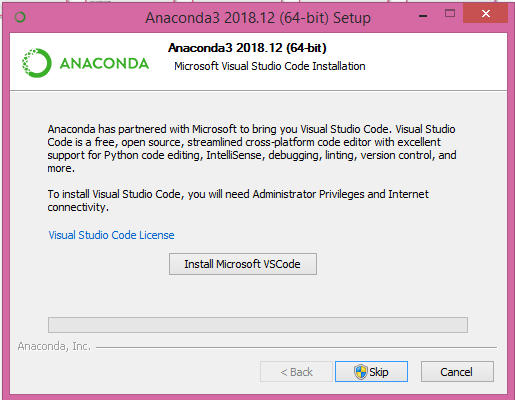
\includegraphics[scale=0.4]{figures/instal/8.PNG}
	  \caption{Instalasi Anaconda Proses 6}
	  \label{labelgambar7}
	  \end{figure}
  \item Setelah selesai, pilih Finish. 
  
\end{enumerate}
\subsection{How to get the Dataset}
